%! TeX root = master.tex
% !TEX program = lualatex

\chapter{Unsupervised Learning}

\lecture{11}{05-05-2026}{Dimensionality Reduction}{}

\section{From supervised to unsupervised learning}
Until now, we have focused on \textbf{supervised learning}, which proceeds in two stages:
\begin{itemize}
  \item \textbf{Training}: use data with ground-truth labels to optimize model parameters by minimizing a loss between predicted and true labels.
  \item \textbf{Testing}: predict the output for new (unlabeled) data samples using the model with fixed parameters.
\end{itemize}
Supervised learning works well when one has a concrete prediction task to solve and labeled
data. It is, however, not suited to scenarios where labels are unavailable, or where the goal is
to \emph{understand} the data rather than predict something about it.

This motivates \textbf{unsupervised learning}, where the goal is no longer prediction but
rather to \textbf{transform the data} for further analysis. There is no ``training/testing''
split: a single algorithm produces a transformed version of the input data.

\section{Dimensionality reduction}
\textbf{Dimensionality reduction (DR)} is our first unsupervised learning task. It is useful for
\begin{itemize}
  \item \textbf{Data visualization}: projecting high-dimensional data into 2D or 3D so it can be plotted and inspected.
  \item \textbf{Data size reduction}: e.g, vectorizing an image yields a huge vector ($x_i \in \mathbb{R}^{536 \cdot 356 \cdot 3} = \mathbb{R}^{572448}$). Dealing with such large data is cumbersome -- can we compress it while keeping the relevant information?
\end{itemize}

\subsection{Intuition: the data manifold}
A $536 \times 536$ RGB image lies in a $\mathbb{R}^{572448}$ space, but so does pure random noise.
The point is that natural images form a tiny subset of this huge space: we are very unlikely to
encounter random noise in the real world. The data of interest typically lies in a much
\textbf{lower-dimensional space} embedded inside the high-dimensional one, called a
\textbf{manifold}.

\textbf{Example}: consider many $32 \times 32$ images obtained by translating
and rotating a single digit $3$. The data lies in a $32 \times 32 = 1024$-dimensional space,
but inherently has only \textbf{3 degrees of freedom} (2 translations and 1 rotation), so it
truly lies on a 3D manifold inside this 1024D space.

Dimensionality reduction is therefore the task of:
\begin{itemize}
  \item Discovering the data manifold.
  \item Getting a low-dimensional representation of the data.
  \begin{itemize}
    \item Sometimes at some loss of information (hopefully noise).
  \end{itemize}
\end{itemize}

\subsection{Formal setting}
Let $x_i \in \mathbb{R}^D$ be a high-dimensional data sample and $y_i \in \mathbb{R}^d$ its
low-dimensional representation, with $d < D$. Our goal is to find a mapping
\[
y_i = f(x_i).
\]
The simplest choice is a \textbf{linear} mapping, $y_i = W^T x_i$. This leads to PCA.
\begin{center}
   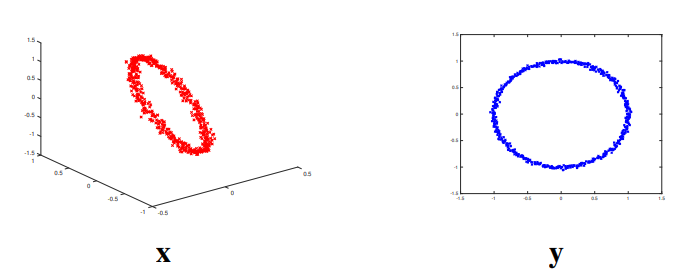
\includegraphics[width=0.7\linewidth]{images/img_20260505_181327.png}
\end{center}


\subsection{Principal Component Analysis (PCA)}
PCA is a linear DR method. Given $N$ samples
$\{x_i\}_{i=1}^{N}$, PCA produces a projection of the form
\[
y_i = W^T (x_i - \bar{x}) \quad \text{s.t.} \quad W^T W = I_d,
\]
where $\bar{x} = \tfrac{1}{N} \sum_{i=1}^{N} x_i$ is the empirical mean of the data.
The data is unsupervised, so we need to clarify what we want this projection to
achieve.

\subsubsection{Objective: variance maximization}
Intuitively, we want to keep most of the ``important'' signal while discarding noise. This can
be achieved by finding directions along which the projected data has \textbf{large variance}:
for the $j$-th output dimension, we want to maximize
\[
\mathrm{var}\bigl(\{y_i^{(j)}\}\bigr) = \frac{1}{N} \sum_{i=1}^{N} \bigl(y_i^{(j)} - \bar{y}^{(j)}\bigr)^2,
\]
where $\bar{y}^{(j)}$ is the mean of the $j$-th dimension of the data after projection.

Maximizing variance means choosing the direction that best preserves the distances between points, 
i.e. the one that makes the projected points as distinguishable as possible — 
which is exactly what we want when compressing information.

\subsubsection{1D projection}
Let us first consider projecting onto a 1D space. We replace the matrix $W \in \mathbb{R}^{D \times d}$
by a single vector $w_{(1)} \in \mathbb{R}^D$ with $\|w_{(1)}\| = 1$. The projected data has mean
\[
\bar{y} = \frac{1}{N} \sum_{i=1}^{N} y_i 
        = \frac{1}{N} \sum_{i=1}^{N} w_{(1)}^T (x_i - \bar{x})
        = w_{(1)}^T \biggl( \frac{1}{N} \sum_{i=1}^{N} x_i \biggr) - w_{(1)}^T \bar{x} = 0,
\]
since the data is centered by construction. The variance after projection then becomes
\[
\mathrm{var}(\{y_i\}) = \frac{1}{N} \sum_{i=1}^{N} (y_i - \bar{y})^2
=\frac{1}{N} \sum_{i=1}^{N} \bigl(w_{(1)}^T (x_i - \bar{x})\bigr - 0)^2 
  \]
  \[
    = \frac{1}{N} \sum_{i=1}^{N}w_{(1)}^T (x_i - \bar{x})(x_i - \bar{x})^T w_{(1)}
= w_{(1)}^T \underbrace{\biggl( \frac{1}{N} \sum_{i=1}^{N} (x_i - \bar{x})(x_i - \bar{x})^T \biggr)}_{C} w_{(1)}
= w_{(1)}^T C w_{(1)},

  \]
where $C \in \mathbb{R}^{D \times D}$ is the \textbf{input data covariance matrix}.

\subsubsection{Constrained optimization via Lagrangian}
We seek to solve
\[
\max_{w_{(1)}} w_{(1)}^T C w_{(1)} \quad \text{s.t.} \quad w_{(1)}^T w_{(1)} = 1.
\]
To do so, we can form the Lagrangian (use to solve optimisation problem with such constraint)
\[
\mathcal{L}(w_{(1)}, \lambda_1) = w_{(1)}^T C w_{(1)} + \lambda_1 \bigl(1 - w_{(1)}^T w_{(1)}\bigr)
\]
and setting its gradient w.r.t. $w_{(1)}$ to zero yields
\[
\boxed{\, C w_{(1)} = \lambda_1 w_{(1)} \,}
\]
which is the definition of an \textbf{eigenvector}: $w_{(1)}$ must be an eigenvector of $C$
with eigenvalue $\lambda_1$. The natural question is: \emph{which one?}

\textbf{Answer}: multiplying both sides on the left by $w_{(1)}^T$ and using the unit-norm
constraint gives
\[
w_{(1)}^T C w_{(1)} = \lambda_1 w_{(1)}^T w_{(1)} = \lambda_1.
\]
The left-hand side is exactly the variance of the projected data. Since we want to
\emph{maximize} it, we should choose $w_{(1)}$ to be the eigenvector corresponding to the
\textbf{largest eigenvalue} of $C$.

\subsubsection{From 1D to $d$-dimensional projections}
For $d > 1$ output dimensions, we proceed \textbf{recursively}:
\begin{itemize}
  \item $w_{(2)}$ is the eigenvector of $C$ with the second largest eigenvalue.
  \item $w_{(3)}$ is the third one, and so on.
\end{itemize}
The projection matrix is obtained by concatenating these eigenvectors as columns:
\[
W = \bigl[\, w_{(1)} \;\; w_{(2)} \;\; \cdots \;\; w_{(d)} \,\bigr] \in \mathbb{R}^{D \times d}.
\]
This automatically satisfies the constraint $W^T W = I_d$, since the eigenvectors of a
(symmetric) matrix are orthogonal and of unit norm.


\subsubsection{Choosing the dimension $d$}
Several options exist:
\begin{itemize}
  \item \textbf{Use all dimensions} ($d = D$): no dimensionality reduction. In 3D, this can be
        seen as a rotation of the data. There is no loss of information, and the dimensions
        in the new space are uncorrelated.
  \begin{center}
     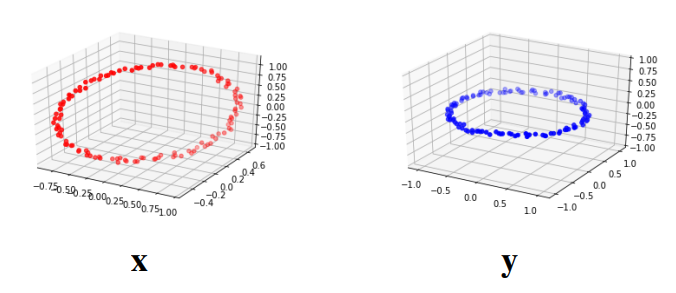
\includegraphics[width=0.7\linewidth]{images/img_20260505_184656.png}
  \end{center}
  
  \item \textbf{Keep all eigenvectors with non-zero eigenvalues}: the data is then truly
        low-dimensional (e.g., when fewer samples than dimensions: $N < D$), and the resulting $\{y_i\}$ have $d < D$
        with no loss of information. 

  \begin{center}
     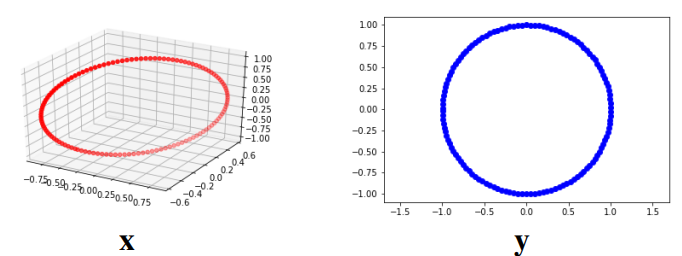
\includegraphics[width=0.7\linewidth]{images/img_20260505_185111.png}
  \end{center}
  
  \item \textbf{Truncate}: in practice, one typically discards some non-zero eigenvalues.
        A common rule is to retain a pre-defined percentage of the data variance, measured as the
        sum of eigenvalues. For instance, to retain at least $90\%$ of the variance, find the
        smallest $d$ such that
        \[
        \sum_{j=1}^{d} \lambda_j \;\geq\; 0.9 \cdot \sum_{k=1}^{D} \lambda_k,
        \]
        with eigenvalues sorted in decreasing order. The resulting $\{y_i\}$ have an even
        lower dimension, at the cost of some loss of information.
  \begin{center}
     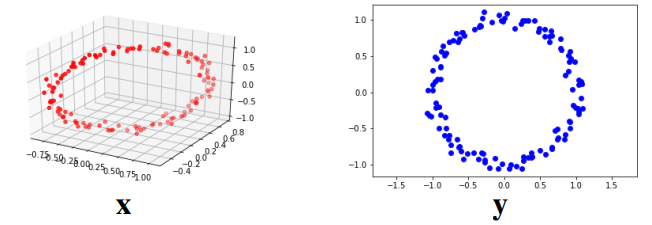
\includegraphics[width=0.7\linewidth]{images/img_20260505_185551.png}
  \end{center}
 Note that even when truncating, the corresponding rectangular matrix $W$ is the
orthogonal matrix that minimizes the reconstruction error
\[
e_i = \|\hat{x}_i - x_i\|^2.
\]
where
\[
\hat{x}_i \;=\; \bar{x} + W y_i \;=\; \bar{x} + W W^T (x_i - \bar{x}),
\]
In other words, for any fixed target dimension $d$, no other orthogonal projection
onto a $d$-dimensional subspace yields a smaller reconstruction error than PCA --
the loss incurred by truncation is the smallest possible at that dimension.

\end{itemize}

\textbf{Remark:}
The maximum dimensionality obtained after PCA is
\[
d_{\max} = \min(N - 1, D),
\]
where $N$ is the number of samples and $D$ is the dimension of the original space.
The $-1$ comes from the fact that we subtract the mean to center the data, which 
costs one degree of freedom.

\subsubsection{PCA as a continuous mapping}
PCA does not only compress the data: it also defines a \textbf{continuous mapping back} from
the low-dimensional space to the high-dimensional one. For any $y \in \mathbb{R}^d$,
\[
\hat{x} = \bar{x} + W y \in \mathbb{R}^D.
\]
This mapping constrains $\hat{x}$ to lie in a $d$-dimensional affine subspace, which acts as
a form of \textbf{regularization}: arbitrary points in the latent (hidden) space ($\mathbb{R}^d$) 
always decode to plausible points on the learned subspace (the $d$-dimensional subspace
embedded in $\mathbb{R}^D$).

\paragraph{Example}
Add a new point on the compressed data to visualize it in the original data representation
\begin{center}
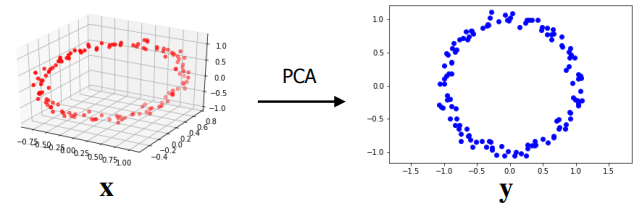
\includegraphics[width=0.5\linewidth]{images/img_20260505_193807.png}
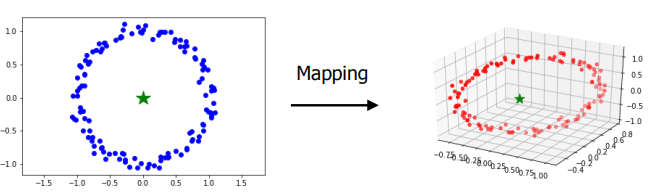
\includegraphics[width=0.5\linewidth]{images/img_20260505_194359.png}
\end{center}

\subsection{Kernel PCA}
PCA is a \textbf{linear} method: it just rotates and projects the data. It cannot ``unroll''
nonlinear structures such as the \emph{Swiss roll}, where a projection would simply squash the
roll instead of unfolding it.
\begin{center}
   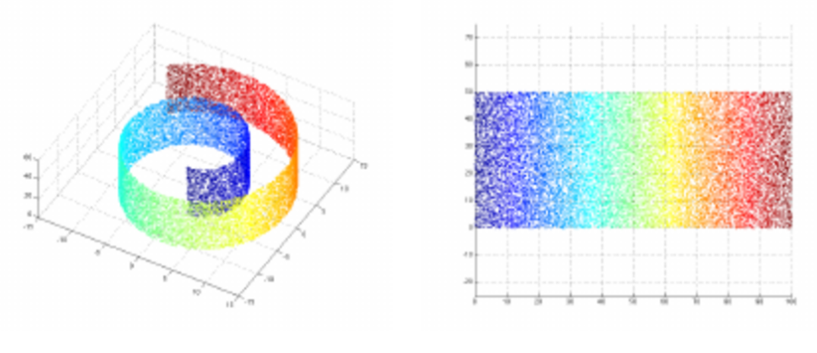
\includegraphics[width=0.5\linewidth]{images/img_20260505_200346.png}
\end{center}


\textbf{Kernel PCA} extends PCA to nonlinear settings using the same
intuition as supervised kernel methods:
\begin{itemize}
  \item Map the data to a high-dimensional feature space, $x_i \mapsto \phi(x_i)$.
  \item Then perform PCA in this feature space.
  \item Replace dot products with kernel evaluations $k(x_i, x_j) = \phi(x_i)^T \phi(x_j)$ to avoid ever computing $\phi$ explicitly.
\end{itemize}

\subsubsection{Derivation (centered case)}
Assume first that the data is centered in feature space: $\frac{1}{N} \sum_{i=1}^{N} \phi(x_i) = 0$.
The covariance matrix in feature space is
\[
C = \frac{1}{N} \sum_{i=1}^{N} \phi(x_i) \phi(x_i)^T \in \mathbb{R}^{F \times F}.
\]
This is an $F \times F$ matrix (not $N \times N$), so it is not directly expressible from
kernel values. PCA in feature space requires solving
\[
C w_{(1)} = \lambda_1 w_{(1)}, \qquad w_{(1)} \in \mathbb{R}^F.
\]
Substituting $C$:
\[
\biggl(\frac{1}{N} \sum_{i=1}^{N} \phi(x_i) \phi(x_i)^T\biggr) w_{(1)} = \lambda_1 w_{(1)}.
\]

By the \textbf{Representer theorem}, $w_{(1)}$ can be expressed as a linear combination of the
$\{\phi(x_i)\}$:
\[
w_{(1)} = \sum_{j=1}^{N} a_j \, \phi(x_j).
\]
Substituting this form into the eigenvector equation and (after some computation, skipped here)
multiplying by $\phi(x_k)^T$ for each $k$ yields a new eigenvalue problem
\[
\boxed{\, K a = \lambda_1 N a \,}
\]
where $a \in \mathbb{R}^N$ contains the new parameters and $K \in \mathbb{R}^{N \times N}$ is
the \textbf{kernel matrix} with entries $K_{ij} = k(x_i, x_j)$.

\subsubsection{From $a$ to projections}
In theory we could recover $w_{(1)} = \sum_{i=1}^{N} a_i \phi(x_i)$, but this depends on the
unknown $\{\phi(x_i)\}$. As in kernel ridge regression, we are not really interested in
$w_{(1)}$ -- we want the low-dimensional projections $\{y_i\}$. For a 1D representation,
\[
y_i = \phi(x_i)^T w_{(1)} = \sum_{j=1}^{N} a_j \, \phi(x_i)^T \phi(x_j) = \sum_{j=1}^{N} a_j \, k(x_i, x_j),
\]
which depends only on the kernel function. As in linear PCA, multiple output dimensions are
obtained by taking the $d$ eigenvectors of $K$ with the largest eigenvalues.

\subsubsection{Non-centered data}
In general, even if the original data is centered, the data in feature space is typically not.
Define the centered feature mapping
\[
\tilde{\phi}(x_i) = \phi(x_i) - \frac{1}{N} \sum_{j=1}^{N} \phi(x_j).
\]
The corresponding kernel matrix $\tilde{K}_{ij} = \tilde{\phi}(x_i)^T \tilde{\phi}(x_j)$ can be
computed directly from the original kernel matrix as
\[
\tilde{K} = K - \mathbf{1}_N K - K \mathbf{1}_N + \mathbf{1}_N K \mathbf{1}_N,
\]
where $\mathbf{1}_N$ is the $N \times N$ matrix with every entry equal to $1/N$. One then runs
the eigenvalue problem on $\tilde{K}$ instead of $K$.

\subsubsection{Examples and intuition}
\begin{itemize}
  \item \textbf{Swiss roll}: linear PCA squashes it; kernel PCA with an RBF kernel can unroll it into a 2D plane.
  \begin{center}
    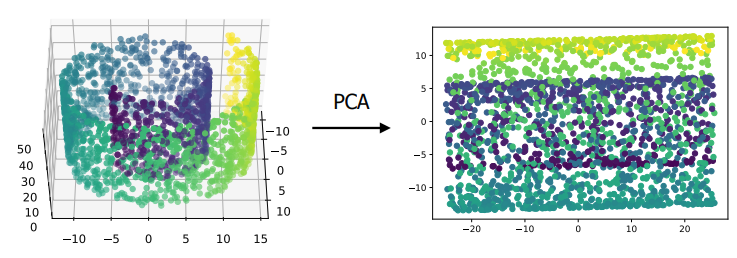
\includegraphics[width=0.49\linewidth]{images/img_20260505_201628.png}
    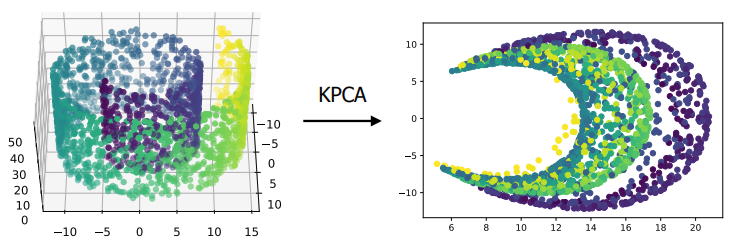
\includegraphics[width=0.49\linewidth]{images/img_20260505_201727.png}
  \end{center}

  \item \textbf{Concentric spheres in 3D} (one inner ``ball'' of class 2 surrounded by an outer ``shell'' of class 1):
    \begin{center}
       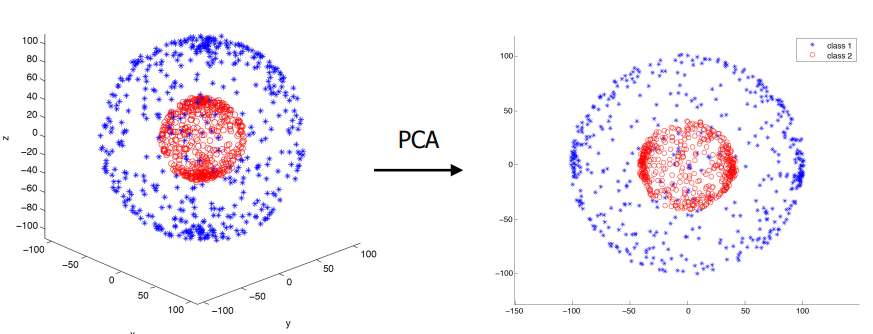
\includegraphics[width=0.49\linewidth]{images/img_20260505_202034.png}
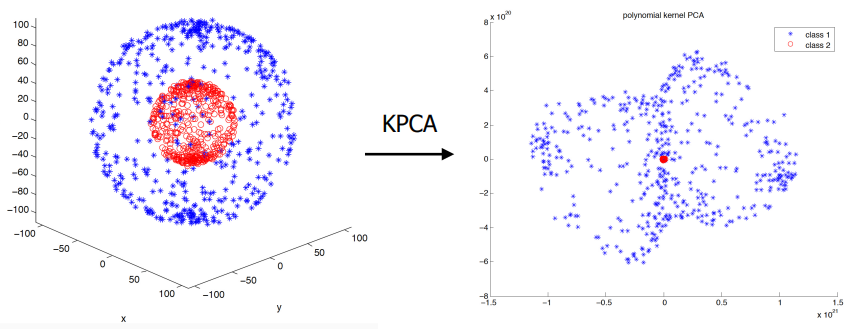
\includegraphics[width=0.49\linewidth]{images/img_20260505_202106.png}
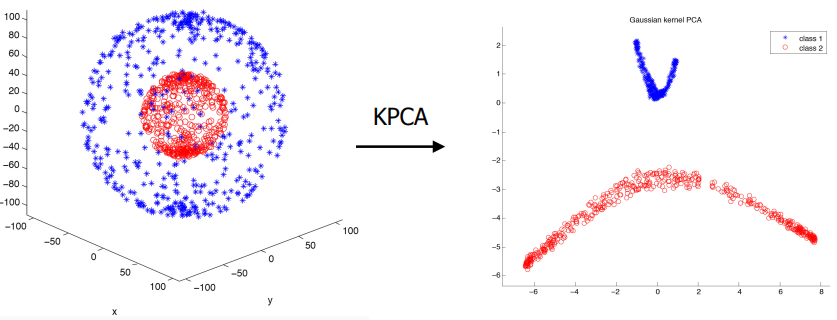
\includegraphics[width=0.5\linewidth]{images/img_20260505_202128.png}
    \end{center}
    
    \begin{itemize}
      \item Linear PCA preserves the nested structure -- classes stay tangled.
      \item Kernel PCA with a polynomial kernel does not separate the classes well either.
      \item Kernel PCA with an \textbf{RBF kernel} cleanly separates the two classes.
    \end{itemize}
  \item \textbf{Why does RBF work here?} The RBF kernel $k(x_i, x_j) = \exp(-\gamma \|x_i - x_j\|^2)$ measures \emph{similarity by distance}. Points within the inner ball are mutually close, points on the outer shell are also mutually close, but inner and outer points are far apart. The kernel essentially encodes ``which group am I close to'', which is exactly the relevant feature here.
\end{itemize}
\vspace{-11pt}
\subsubsection{Kernel PCA vs PCA: the missing inverse mapping}
\begin{itemize}
  \item Both PCA and kernel PCA give a mapping from high to low dimension.
  \item PCA \textbf{also} provides a clean inverse mapping $\hat{x} = \bar{x} + Wy$ from low back to high dimension.
  \item \textbf{Kernel PCA does not}: there is no direct way to compute the high-dimensional version of an arbitrary point in the low-dimensional space (the inverse of $\phi$ is not available in general).
\end{itemize}
This raises the question: can we have a \emph{nonlinear} method that \emph{also} provides an
inverse mapping? The answer leads us to autoencoders.

% --- SCHEMAS À AJOUTER : ---
% - Slide 47 : Swiss roll (3D -> 2D unrolled)
% - Slide 56/57 : Swiss roll PCA vs Kernel PCA (RBF)
% - Slide 58/59/60 : 3D nested spheres, PCA / poly-KPCA / RBF-KPCA

\subsection{Autoencoders}
\subsubsection{From PCA to autoencoders}
PCA provides two linear mappings:
\[
y = W^T (x - \bar{x}), \qquad \hat{x} = \bar{x} + W y.
\]
Because both are linear, PCA cannot handle nonlinearly-structured data such as the Swiss roll.
There is no fundamental reason to restrict ourselves to linear mappings.

\begin{wrapfigure}{r}{0.3\linewidth}
  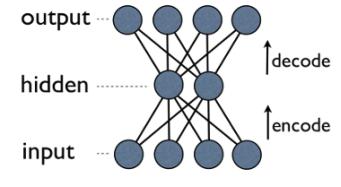
\includegraphics[width=\linewidth]{images/img_20260505_202646.png}
\end{wrapfigure}

The simplest nonlinear extension is to insert an \textbf{element-wise nonlinear activation
function} $f(\cdot)$ in the middle, giving
\[
\hat{x} = W f(W^T x).
\]
This is the basic form of an \textbf{autoencoder}.

\subsubsection{General form}
More generally, an autoencoder consists of two mappings:
\begin{itemize}
  \item The \textbf{encoder} maps the input $x$ to a latent representation (or \emph{code}) $y$.
  \item The \textbf{decoder} maps the latent representation back to an output $\hat{x}$ in the same space as $x$.
\end{itemize}
\begin{center}
   
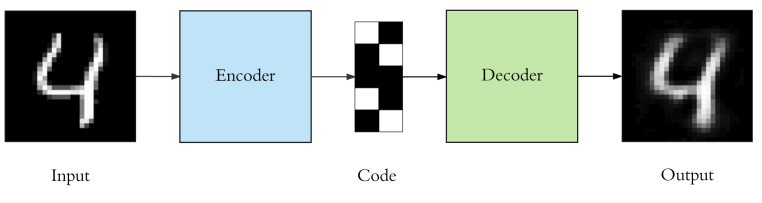
\includegraphics[width=0.6\linewidth]{images/img_20260505_202909.png}
\end{center}

As in PCA, the output of the decoder is meant to be similar to the original input.

\subsubsection{Deep autoencoders}
There is no reason to restrict the encoder and decoder to a single layer. Stacking multiple
layers (each with its own activation) yields a \textbf{deep autoencoder}. Each layer
implements
\[
z_{(j)} = f_{(j)}\!\bigl( W_{(j)}^T \, z_{(j-1)} \bigr),
\]
with $z_{(0)} = x$ on the encoder side, and the latent code is the innermost activation. The
decoder typically mirrors the encoder structure.
\begin{center}
   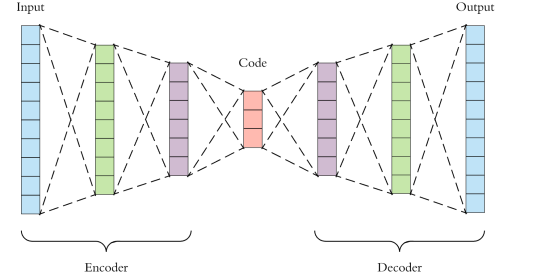
\includegraphics[width=0.6\linewidth]{images/img_20260505_203029.png}
\end{center}

\subsubsection{Training}
Following the PCA reconstruction-error perspective, an autoencoder is trained by minimizing the \textbf{empirical reconstruction
risk}
\[
R(\{W_{(j)}\}) = \frac{1}{N} \sum_{i=1}^{N} \bigl\| \hat{x}_i(\{W_{(j)}\}) - x_i \bigr\|^2.
\]
Like for MLPs, this objective is non-convex, and minimization is performed via
\textbf{stochastic gradient descent} with backpropagation.

\subsubsection{Dimensionality expansion and the trivial solution}
With a linear mapping (PCA), reducing dimensionality is mandatory to do something interesting:
keeping $d = D$ would simply rotate the data. With a \textbf{nonlinear} mapping, this
restriction disappears, and one can even \textbf{expand} the latent dimensionality to be larger
than the input dimension.

This raises a problem: with enough capacity, an autoencoder can simply learn the
\textbf{identity} mapping (just copying the input), which is useless. Two main strategies
prevent this trivial solution.

\subsubsection{Denoising autoencoders}
Add noise to the input but ask the network to reconstruct the \textbf{clean} (noise-free)
version of the input. The network then has to learn the structure of the data manifold to
remove noise rather than just copying. This forces the latent representation to capture
meaningful structure.
\begin{center}
   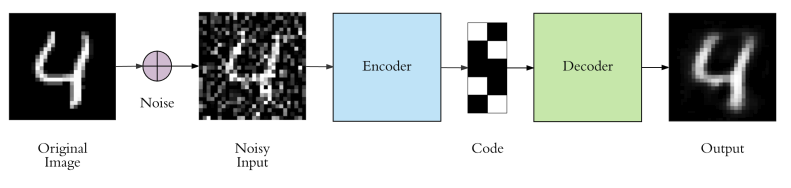
\includegraphics[width=0.8\linewidth]{images/img_20260505_203608.png}
\end{center}

\subsubsection{Sparse autoencoders}
The idea is to force the latent code to be \textbf{sparse}, i.e., to have most of its 
components equal to zero, with only a few non-zero ones. With limited "active" components, 
the network cannot trivially copy the input across all latent units -- it must instead 
learn a representation where each active component captures something meaningful.

Letting $y_i \in \mathbb{R}^M$ be the code for sample $i$, sparsity is encouraged by adding 
an $L_1$ penalty to the reconstruction loss:
\[
E_r(\{W_{(j)}\}) = \sum_{i=1}^{N} \sum_{k=1}^{M} \bigl| y_i^{(k)} \bigr|.
\]
The total training objective then becomes
\[
\mathcal{L} = \underbrace{\frac{1}{N} \sum_{i=1}^{N} \|\hat{x}_i - x_i\|^2}_{\text{reconstruction}} 
\;+\; \beta \cdot \underbrace{\sum_{i=1}^{N} \sum_{k=1}^{M} |y_i^{(k)}|}_{\text{sparsity}},
\]
where $\beta > 0$ controls the strength of the sparsity constraint.

\textbf{Why $L_1$ and not $L_2$?} The $L_1$ norm has the special property of producing 
\emph{exactly zero} components at the optimum, while $L_2$ would only shrink them towards 
small values without setting them to zero. This makes $L_1$ the natural choice for inducing 
true sparsity.

The two terms compete: reconstruction wants to use as many components as needed for fidelity, 
while sparsity wants to silence as many as possible. The network is therefore forced to use 
each active component efficiently -- it must encode the most informative features rather than 
trivially copying the input.\subsubsection{Convolutional autoencoders}
For image data, the encoder and decoder can be built from convolutional layers (encoder) and
upsampling-convolutions or transposed convolutions (decoder) -- mirroring the FCN/U-Net idea
seen in Lecture 10. Fully-connected layers are often inserted at the bottleneck. (E.g, Guo et
al., ICONIP 2017.)
\begin{center}
   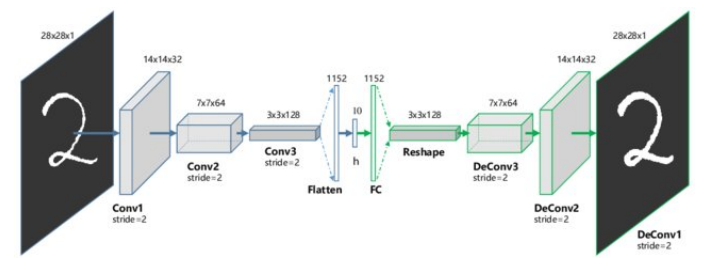
\includegraphics[width=0.7\linewidth]{images/img_20260505_204407.png}
\end{center}

\subsubsection{Applications}
\begin{itemize}
  \item \textbf{Compact representation / retrieval}: the latent code is a compact summary of the input. Retrieval in a large data collection can be done by $k$-nearest neighbors in code space (e.g, image retrieval).
  \begin{center}
     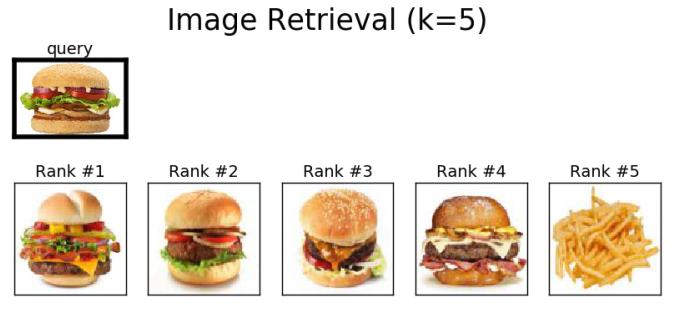
\includegraphics[width=0.5\linewidth]{images/img_20260505_204605.png}
  \end{center}
  
  \item \textbf{Generative use of the decoder}: as in PCA, the decoder defines a mapping from the latent space to the output (same as input) space. By picking arbitrary points in the latent space (we input directly in the latent space), one can generate new samples (e.g, new digit-like images). This is a stepping stone toward proper generative models.
  \begin{center}
    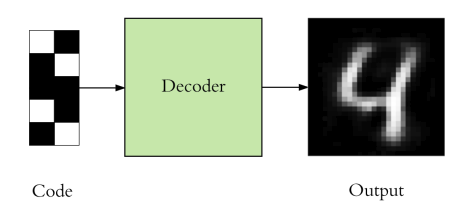
\includegraphics[width=0.5\linewidth]{images/img_20260505_204910.png}
  \end{center}
\end{itemize}

\clearpage
